\section{Performance Regression Analysis}
\label{src:regression}
As there are no restrictions on the number of allowed partitions per
memory kind, it is legal to create \texttt{SHMEM\_MAX\_PARTITIONS}
on a single kind of memory. This section details the performance
regression analysis on the following two scenarios using Cray SHMEM
version 7.6.0:
\begin{itemize}
    \item Using symmetric heap created on default partition instead of
    the existing \texttt{SMA\_SYMMETRIC\_SIZE} environment variable; and
    \item Creating \texttt{SHMEM\_MAX\_PARTITIONS} number of partitions.
\end{itemize}

\subsection{Using default partition instead of
\texttt{SMA\_SYMMETRIC\_SIZE}}
\label{src:regression/partition1}
As mentioned in Section~\ref{src:smempart/part1} the default partition
has a special functionality. To provide backward compatibility in
existing legacy applications, the symmetric heap created
from the default partition is used for \texttt{shmem\_malloc} and
\texttt{shmem\_align} routines. Hence, in this section we analyzed the
performance regression specifically on using the default partition.

\begin{figure*}[ht!]
    \vspace{-20pt}
    \centering
    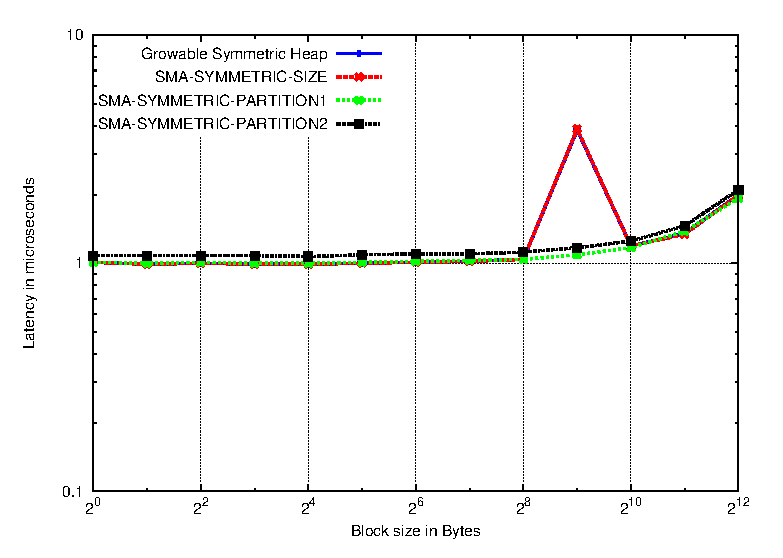
\includegraphics[width=\linewidth]{graph/partition1-bdw.eps}
    \caption{Performance of OSU Put Microbenchmark in using source and
    destination buffers allocated using symmetric heaps created from
    different options
    %\texttt{SMA\_SYMMETRIC\_SIZE}, \texttt{SMA\_SYMMETRIC\_PARTITION1},
    %\texttt{SMA\_SYMMETRIC\_PARTITION2} environment variables and the
    %default growable symmetric heap
    on Cray XC system with Intel Broadwell
    processors}
    \label{graph:partition1-bdw}
    \vspace{-15pt}
\end{figure*}

\begin{figure*}[ht!]
    %\vspace{-20pt}
    \centering
    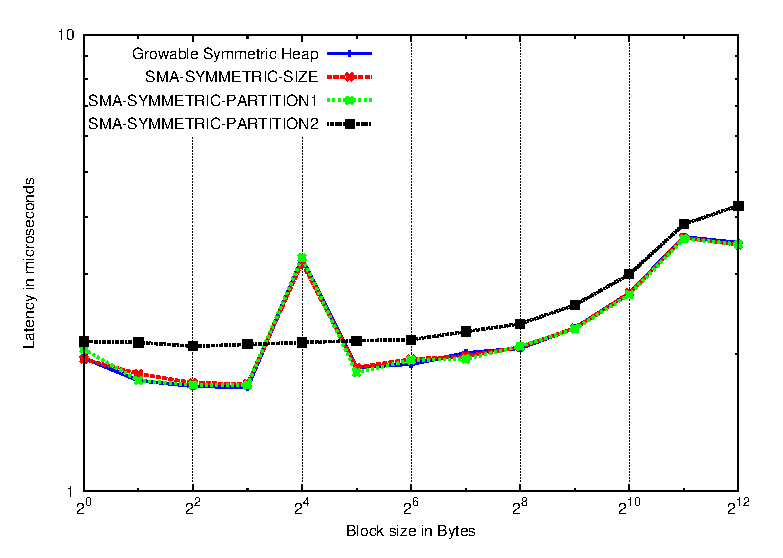
\includegraphics[width=\linewidth]{graph/partition1-knl.eps}
    \caption{Performance of OSU Put Microbenchmark in using source and
    destination buffers allocated using symmetric heaps created from
    different options
    %\texttt{SMA\_SYMMETRIC\_SIZE}, \texttt{SMA\_SYMMETRIC\_PARTITION1},
    %\texttt{SMA\_SYMMETRIC\_PARTITION2} environment variables and the
    %default growable symmetric heap
    on Cray XC system with Intel KNL
    processors}
    \label{graph:partition1-knl}
    \vspace{-30pt}
\end{figure*}

Fig.~\ref{graph:partition1-bdw} and Fig.~\ref{graph:partition1-knl}
shows the performance of OSU put microbenchmark with symmetric heaps
created from the following three options on Intel Broadwell and Intel
KNL processor based Cray XC systems respectively:
\begin{itemize}
    \item Symmetric heap created with the size determined from
    \texttt{SMA\_SYMMETRIC\_SIZE} environment variable;
    \item Symmetric heaps on partitions defined using
    \texttt{SMA\_SYMMETRIC\_PARTITION} environment variable; and
    \item In Cray SHMEM, if both \texttt{SMA\_SYMMETRIC\_SIZE} and a
    default partition is not specified, then a default symmetric heap
    grows dynamically as needed to a maximum of 2 GB per PE.
\end{itemize}

From Fig.~\ref{graph:partition1-bdw} and
Fig.~\ref{graph:partition1-knl}, we see that the performance of
\texttt{shmem\_putmem} operation on symmetric heap allocations
using the environment variables is almost identical to allocations
on the growable symmetric heap in both Intel Broadwell
and KNL processor based systems. But, the performance on symmetric
heap from partitions other than the default partition is about 5\%
less on Intel Broadwell based systems and about 7\% less than
Intel KNL based systems.

%Symmetric heap maintenance
%includes memory registration with NIC.% and offset maintenance on
%each PE.
%Though upcoming communication layers like
%libfabrics~\cite{libfabrics} have support for Scalable memory
%registration, Cray SHMEM implementation over DMAPP uses basic memory
%registration. Hence there is an increase in memory footprint on
%DMAPP on maintaining symmetric heaps on each PE.

%Apart from increase in memory footprint on memory registration,
%Hence, in our
%performance regression test, we analyzed the performance of

\begin{figure*}[ht!]
    \vspace{-25pt}
    \centering
    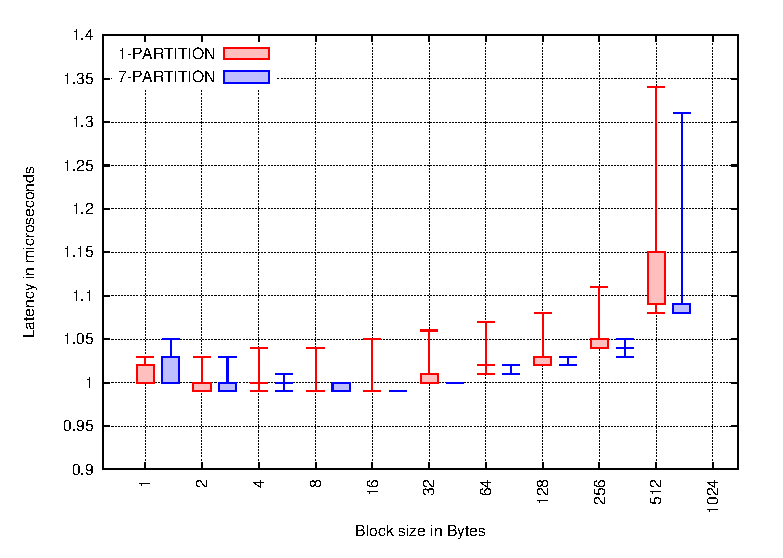
\includegraphics[width=\linewidth]{graph/osu-put.eps}
    \caption{Performance difference on using destination buffers
    from 1 partition against 6 partitions in the modified OSU Put
    microbenchmark on Intel KNL based Cray XC system using 2 PEs
    with 1 PE per node}
    \label{graph:lookup}
    \vspace{-30pt}
\end{figure*}

\subsection{Creating \texttt{SHMEM\_MAX\_PARTITIONS} partitions}
\label{src:regression/max}
Creating multiple symmetric memory partitions results in
multiple symmetric heaps on each PE.
Identifying the correct symmetric segment is essential before
performing an
underlying communication operation. %with symmetric heap lookup on each
%RMA and AMO operation is expected to introduce performance
%regression.
Algorithm~\ref{algo:normal-lookup} shows the introduction of lookup
logic trying to match the correct symmetric heap segment on the
\texttt{shmem\_putmem} operation. Similar, lookups are introduced on
all OpenSHMEM RMA and AMO operations. \texttt{USER\_SEGMENT} refers to
the symmetric heaps created on user-defined memory partitions.

%\vspace{-20pt}
\begin{algorithm}[ht!]
\begin{algorithmic}
    \Procedure{\texttt{shmem\_putmem}}
    {void *dest, const void *src, size\_t nblks, int pe\_id}\;
        dmapp\_seg\_desc\_t *target\_seg = \texttt{NULL}\;
        dmapp\_type\_t type = \texttt{DMAPP\_BYTE}\;
        \If {\normalfont (dest.segment $\equiv$
                         \texttt{DATA\_SEGMENT})} {
            target\_seg = \texttt{DATA\_SEGMENT}\;
            \tcp{verify if dest buffer is a static or global variable}
        } \ElseIf {\normalfont (dest.segment $\equiv$
                         \texttt{SHEAP\_SEGMENT})} {
            target\_seg = \texttt{SHEAP\_SEGMENT}\;
            \tcp{verify if dest buffer is in default symmetric heap}
        } \Else {
            segment\_identified = \textit{false}\;
            \For {\normalfont (int i = 1; i $\leq$ N; i++)}{
                \If{\normalfont (dest.segment $\equiv$
                    \texttt{USER\_SEGMENT\_i})} {
                    target\_seg = \texttt{USER\_SEGMENT\_i})\;
                    segment\_identified = \textit{true}\;
                }
            }
            \If{\normalfont(segment\_identified $\equiv$
                    \textit{false})} {
                abort()\;
            }
            \tcp{search through all partitions to match the symmetric heap}
        }
        dmapp\_put(dest, target\_seg, pe\_id, src, nelems, type)\;
        return\;
    \EndProcedure
    \caption{Lookup logic with N symmetric memory partitions per PE}
    \label{algo:normal-lookup}
\end{algorithmic}
\end{algorithm}
%\vspace{-20pt}

We measured the performance regression behind this additional lookup
operation using a modified OSU microbenchmark~\cite{osu-mb}
on a Cray XC system with Intel KNL processors. To measure the average
latency on every \texttt{shmem\_putmem} operation, we use 2 nodes
with 1 PE per node.
The normal OSU microbenchmark selects the buffer from either
\texttt{DATA\_SEGMENT} or \texttt{SHEAP\_SEGMENT}
per job. We modified the benchmark by creating
one destination buffer for \texttt{N} partitions and randomly selected
the destination buffer from different partitions for every iteration.
We timed the average performance of all iterations.% of the
%\texttt{shmem\_putmem} operation.

Fig.~\ref{graph:lookup} shows the
performance difference between using 1 and 6 partitions on very small
data sizes. The average performance variations is around 2\% to
3\%. This can be attributed as noise. If we increase
the number of partitions to 127, we could see variations as high
as 6\%. But, we expect users to create only one partition per
memory kind.
%and not \texttt{N} unnecessary partitions.
Moreover, as mentioned in
Table~\ref{tab:const} the \texttt{SHMEMX\_MAX\_PARTITIONS} library
constant in Cray SHMEM is 7.

We observe similar performance variations on small data sizes on other
RMA and AMO operations. For larger message sizes, the segment lookup
does not contribute for any performance variations.

\section{Performance Analysis}
\label{src:perf}

\begin{figure*}[ht!]
    \vspace{-30pt}
    \centering
    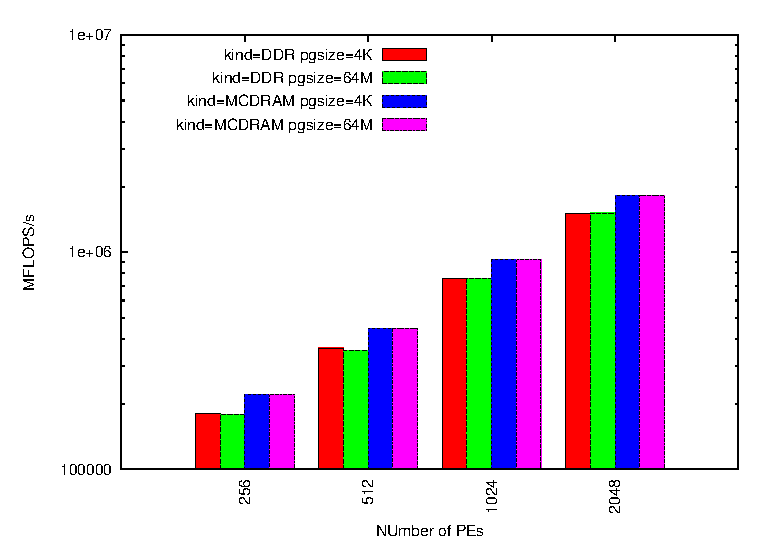
\includegraphics[width=\linewidth]{graph/2d-stencil.eps}
    \caption{Performance difference on using different kinds of memory
    and different hugepages on ParRes 2D-Stencil SHMEM kernels}
    \label{graph:2dstencil}
    \vspace{-20pt}
\end{figure*}

Section~\ref{src:regression} shows the performance impact of
creating multiple partitions. This section details the performance
impact of creating partitions on different kinds of memory using
Cray SHMEM version 7.6.0 on Intel KNL based Cray XC system. We used
a maximum of 64 KNL nodes with 32 PEs per node for our test.

We used ParRes 2D-Stencil SHMEM kernel to analyze the performance
of defining partitions with different kinds of memory and
page sizes. The symmetric heap on the 2D-Stencil kernel fits inside
a single kind of memory and hence we just used default partition. We
used the following configurations for the default partition:
\begin{itemize}
    \item \texttt{NORMALMEM}(DDR) with page size 4K;
    \item \texttt{NORMALMEM}(DDR) with page size 64M;
    \item \texttt{FASTMEM}(DDR) with page size 4K; and
    \item \texttt{FASTMEM}(DDR) with page size 64M;
\end{itemize}
From Fig.~\ref{graph:2dstencil}, we see that the use of MCDRAM
provides around 25\% performance improvement compared against
using DDR. But, for this particular benchmark there is no performance
impact on using different page sizes.

%\begin{figure*}[t!]
%\centering
%    \begin{subfigure}[t]{0.50\textwidth}
%        \centering
%        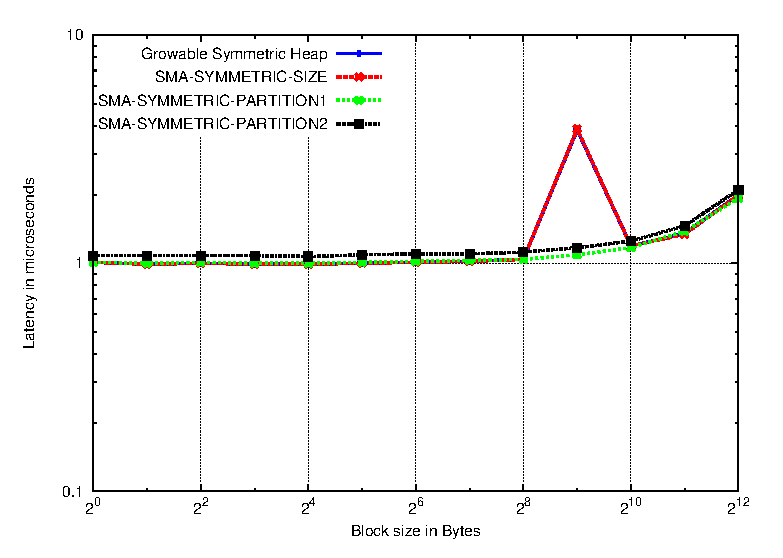
\includegraphics[width=\linewidth]{graph/partition1-bdw.eps}
%        \caption{On Intel Broadwell Systems}
%    \end{subfigure}~~
%    \begin{subfigure}[t]{0.50\textwidth}
%        \centering
%        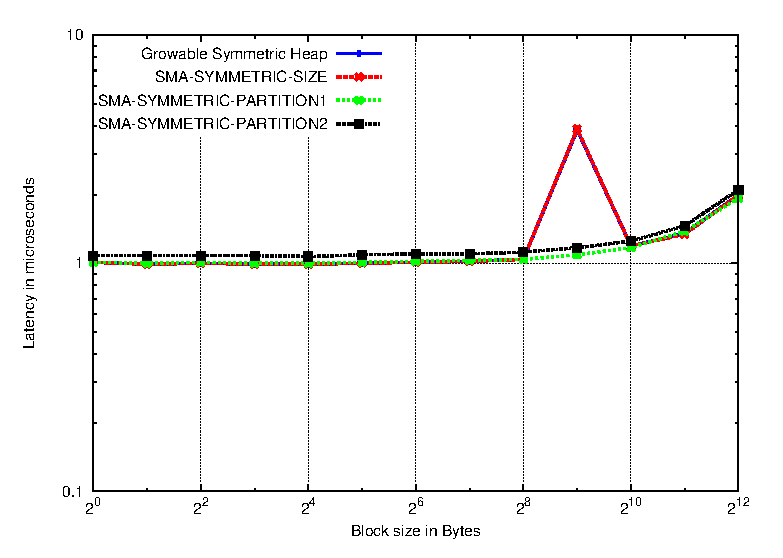
\includegraphics[width=\linewidth]{graph/partition1-bdw.eps}
%        \caption{With and Without Locks for Communication}
%    \end{subfigure}
%    \vspace{-10pt}
%    \caption{Analysis of \texttt{SHMEM\_THREAD\_MULTIPLE} Implementation
%in Modified OSU Put Microbenchmarks on 2 PEs from 2 Separate Nodes}
%    \label{graph:partition1}
%    \vspace{-20pt}
%\end{figure*}


